\documentclass{report}

\input{~/latex/template/preamble.tex}
\input{~/latex/template/macros.tex}

\title{\Huge{Chapter 1 - Differentiation}}
\author{\huge{Matt Warner}}
\date{\huge{}}
\pagestyle{fancy}
\fancyhf{}
\rhead{}
\lhead{\leftmark}
\cfoot{\thepage}
% \usepackage[default]{sourcecodepro}
% \usepackage[T1]{fontenc}


\pgfpagesdeclarelayout{boxed}
{
  \edef\pgfpageoptionborder{0pt}
}
{
  \pgfpagesphysicalpageoptions
  {%
    logical pages=1,%
  }
  \pgfpageslogicalpageoptions{1}
  { 
    border code=\pgfsetlinewidth{1.5pt}\pgfstroke,%
    border shrink=\pgfpageoptionborder,%
    resized width=.95\pgfphysicalwidth,%
    resized height=.95\pgfphysicalheight,%
    center=\pgfpoint{.5\pgfphysicalwidth}{.5\pgfphysicalheight}%
  }%
}

\pgfpagesuselayout{boxed}

\begin{document}
  \maketitle
  \tableofcontents
  \pagebreak
\section{Limits: A numerical and Graphical Approach}
\bigbreak \noindent \bigbreak \noindent
\begin{minipage}{0.44\textwidth}
Consider the pattern formed by the following sequence of numbers	
$$ 0.9, 0.99, 0.999, 0.9999, \text{ and so on}$$
\bigbreak \noindent \bigbreak \noindent
The numbers appear to be getting closer to the number 1, yet never equal 1 exactly. Assuming that the sequence continues in the same manner, we could say that the \textit{limit} of this sequence of numbers is 1. Note that this sequence of numbers approaches 1 ``from the left,'' meaning that all numbers in the sequence are less than the limit, 1. We write $x \rightarrow a $, read ``x approaches a from the left'', to represent a sequence of numbers that approaches $a$ from the left.
\vspace{2mm}

Thus, the sequence 0.9, 0.99,0.999, and so on, is written $x \rightarrow 1$
\end{minipage}
\begin{minipage}{0.55\textwidth}
  \vspace{15mm}
% \begin{figure}[ht]
% \centering
% 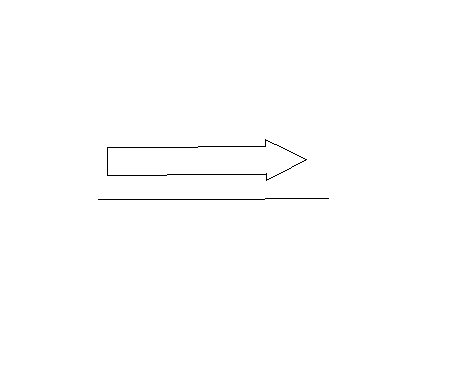
\includegraphics[width=0.5\textwidth]{ /home/mattw/niu/Math211/figures/figfig.pdf}
% \end{figure}
    \bigbreak \noindent
\end{minipage}
\bigbreak \noindent \bigbreak \noindent
    The following sequence approaches 1 ``from the right'':
    $$1.1, 1.01,1.001,1.0001,1.00001, \text{ and so on}$$
    \bigbreak \noindent
    We write $ x \rightarrow a^+$, read ``x approaches $a$ from the right'' to represent a sequence of numbers that approaches $a$ from the right.
    \bigbreak \noindent
    Thus, the sequence 1.1, 1.01,1.001,1.0001,1.00001, and so on, is written $x \rightarrow 1^+$
    \bigbreak \noindent
    \bigbreak \bigbreak \noindent
    \ex{}{
      For each sequence, determine its limit, and rewrite the sequence in the form $x \rightarrow a^-$ or $ x \rightarrow a+$
      \bigbreak \noindent
      \begin{enumerate}
        \item $2.24, 2.249, 2.2499, 2.24999,\ldots$ 
        \item $5.51,5.501,5.5001,5.50001,\ldots$
        \item $\frac{1}{2}, \frac{3}{4}, \frac{7}{8}, \frac{15}{16},\frac{31}{32},\frac{63}{64}$
      \end{enumerate}
    }
    \sol{}
  \bigbreak \noindent
  a) $ x \rightarrow 2.25^-$
  \bigbreak \noindent
  b) $x \rightarrow 5.5^+$
  \bigbreak \noindent
  $ c) x \rightarrow 1^-$
\pagebreak
\subsection{Numerical Limits of Functions}
\bigbreak \noindent
\begin{minipage}[t]{0.46\textwidth}
Suppose $f(x) = 2x + 1$, and let $x$ assume the values in the sequence $0.9,0.99,0.999,0.9999,0.99999$, and so on. Evaluating $f(x)$ for each of these values, we have
$$f(0.9) = 2(0.9) + 1 = 2.8$$
$$f(0.99) = 2(0.99) + 1 = 2.98$$
$$f(0.999) = 2(0.999) + 1 = 2.998$$
$$f(0.9999) = 2(0.9999) + 1 = 2.9998 \text{ and so on.}$$
\bigbreak \noindent
As x approaches the number 1 from the left, the sequence of outputs, $f(x)$, approaches the number 3. This is an example of a \textit{left hand limit} and is written
$$\lim_{x\to 1^-}f(x) = 3$$
\end{minipage}
\hspace{.2in}
\begin{minipage}[t]{0.5\textwidth}
  \vspace{-8mm}

  \thm{}{
As $x$ approaches $a$, the limit of $f(x)$ is $L$, where $L$ is a real number, if the left-hand limit exists and the right-hand limit exists and if both limits are $L$. That is,
$$
\text { if } \lim _{x \rightarrow a^{+}} f(x)=\lim _{x \rightarrow a^{-}} f(x)=L \text {, then } \lim _{x \rightarrow a} f(x)=L .
$$
The converse of this theorem is also true: If $\lim _{x \rightarrow a} f(x)=L$, then it follows that $\lim _{x \rightarrow a^{-}} f(x)=L$ and $\lim _{x \rightarrow a^{+}} f(x)=L$
\vspace{4mm}

If the left-hand or right-hand limit does not exist, or if the right-hand and left-hand limits exist but are different, then the limit itself does not exist.
  }
\end{minipage}
\bigbreak \noindent
\nt{
  writing $x\to 1$ with no superscript, $^+$ or $^-$ on 1 indicates that ``x approaches 1 from \textbf{both sides}'' if both the left-hand limit and the right-hand limit exist and are equal to the same real number $L$, then the \textit{general limit} (or simply, the \textit{limit}) is $L$. In the above example, since the limit as x approaches from both sides is the same. You can ingore writing the superscripts. This leads to theorem 1.
}
\bigbreak \noindent\bigbreak \noindent
\subsection{Graphical Limits}
\bigbreak \noindent
To view limits Graphically, we let $f(x) = 2x+3$ and select x-values that get close to 4. In the table and graph below, we see that as input values approach 4 from the left (that is, are less than 4), output values approach 11, and as input values approach 4 from the right (that is, are greater than 4), output values also approach 11. Thus, we say;
\bigbreak \noindent
As x approaches 4 from either side, the function $f(x) = 2x+3$ approaches 11.
\begin{figure}[ht]
    \centering
    \incfig[1]{lim}
\end{figure}
\bigbreak \noindent
\begin{center}
\begin{tabular}{|c|r|r|r|r|r|r|r|}
  \hline
$x$ & 3.9 & 3.99 & 3.999 & 4 & 4.001 & 4.01 & 4.1 \\
\hline$f(x)$ & 10.8 & 10.98 & 10.998 & 11 & 11.002 & 11.02 & 11.2 \\
\hline
\end{tabular}
\end{center}

\pagebreak
\ex{}{
  Let $f(x) = -3x + 4$. Find the following limits
  \begin{enumerate}
    \item $\displaystyle\lim_{x\to 2^-}f(x)$
    \item $\displaystyle\lim_{x\to2^+}f(x)$
    \item $\displaystyle\lim_{x\to2}f(x)$

      \vspace{3mm}


  \end{enumerate}
}
\bigbreak \noindent
\sol{}
\bigbreak \noindent

$$\displaystyle\lim_{x\to2^-}-3x+4$$
\noindent set x = 2
$$\displaystyle\lim_{x\to2^-}-3(2) +4 = -2$$
\vspace{2mm}

\noindent
Thus the limit of $f(x)$ as x approaches 2 is $-2$
\bigbreak \noindent
The same proccess can be applied to the limit of f(x) as x approaches to the right, since we get the same answer for both, we conclude that
$$\displaystyle\lim_{x\to 2}f(x) = -2$$
\nt{
  The method used above is a shortcut and is only permissible under certain conditions, This will be discussed in the next section. The numerical apporach to finding the limit can be found below.
}
\bigbreak \noindent
a) We choose values of $x$ that approach 2 from the left, and evaluate $f(x)$ :
$$
\begin{aligned}
f(1.9) & =-3(1.9)+4=-1.7, \\
f(1.99) & =-3(1.99)+4=-1.97, \\
f(1.999) & =-3(1.999)+4=-1.997, \text { and so on. }
\end{aligned}
$$
We see that as $x$ approaches 2 from the left, the function values approach -2 . Thus, we have a left-hand limit, $\lim _{x \rightarrow 2} f(x)=-2$
\bigbreak 
b) We choose values of $x$ that approach 2 from the right, and evaluate $f(x)$ :
$$
\begin{aligned}
f(2.1) & =-3(2.1)+4=-2.3, \\
f(2.01) & =-3(2.01)+4=-2.03, \\
f(2.001) & =-3(2.001)+4=-2.003, \text { and so on. }
\end{aligned}
$$
We see that as $x$ approaches 2 from the right, the function values approach -2 . Thus, we have a right-hand limit, $\lim _{x \rightarrow 2^{+}} f(x)=-2$.
\bigbreak \noindent
c) Since the left-hand limit and the right-hand limit exist and are both equal to -2 , we conclude that the limit as $x$ approaches 2 exists and is -2 : $\lim _{x \rightarrow 2} f(x)=-2$.
\pagebreak
\ex{}{
  Let $f(x) = \frac{x^2-1}{x-1}$. Find $\displaystyle\lim_{x\to 1}f(x)$
}
\sol
\bigbreak \noindent
For this question, note that we cannot directly find the limit by setting $x = 1$ (direct substitution), since that would give us a zero in the denominator, which is no good.
\bigbreak
\noindent Thus, we use a numerical approach for this question.
\bigbreak \noindent \bigbreak \noindent
\hspace{25mm}\begin{minipage}{0.45\textwidth}
  \hspace{2em}
  left-hand limit
  \vspace{2mm}

\begin{tabular}{|c|l|}
\hline$x \rightarrow 1^{-}(x<1)$ & $f(x)$ \\
\hline 0.9 & 1.9 \\
0.99 & 1.99 \\
0.999 & 1.999 \\
\hline
\end{tabular}
\vspace{4mm}

\hspace{8mm}$\displaystyle\lim_{x\to 1^-}f(x) = 2$
\end{minipage}
\begin{minipage}{0.39\textwidth}
  \hspace{6mm}right-hand limit
  \vspace{2mm}

	\begin{tabular}{|c|l|}
\hline$x \rightarrow 1^{+}(x>1)$ & $f(x)$ \\
\hline 1.1 & 2.1 \\
1.01 & 2.01 \\
1.001 & 2.001 \\
\hline
\end{tabular}
\vspace{4mm}

\hspace{10mm}$\displaystyle\lim_{x\to 1^+ }f(x) = 2$
\end{minipage}
\bigbreak \noindent
Since the left-hand limit and right-hand limit exist and are equal, we conclude that the limit of $f(x)$ as $x$ approaches 1 is
$$\displaystyle\lim_{x\to 1}f(x) = 2$$
\bigbreak \noindent
Thus, the graph of $f(x) = \frac{x^2-1}{x-1}$ is the line given by $f(x) = x + 1$ where the point corresponding to x = 1 has been removed.
\bigbreak \noindent
The graph has a ``hole'' at the point (1,2). Thus, even though the function is not defined at x = 1, the limit \textit{does} exist as $x\to 1$, and its value is 2.
\begin{figure}[ht]
    \centering
    \incfig[1]{limlim}
    %\caption{limlim}
    %\label{fig:limlim}
\end{figure}
\bigbreak \noindent
To Summarize:
\begin{enumerate}
  \item When x = 1 exactly, $f(x)$ is undefined. The value $x = 1$ is not in the domain of $f$.
  \item When x approaches 1 from both sides, the output values approach 2.
\end{enumerate}
\pagebreak
\ex{}{
  Consider the function $H$ given by
 $$H(x)= \begin{cases}2 x+2, & \text { for } x<1 \\ 2 x-4, & \text { for } x \geq 1\end{cases}$$
 \bigbreak \noindent
 Find $\displaystyle\lim_{x\to 1}H(x)$
}
\sol{}
\bigbreak \noindent
\begin{figure}[ht]
\centering
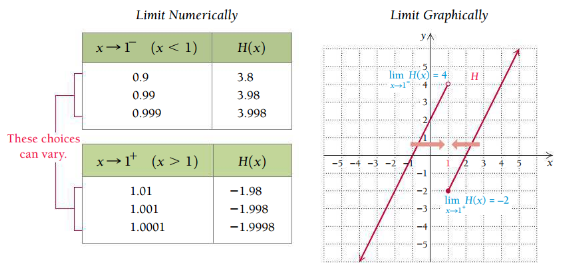
\includegraphics[width=0.7\textwidth]{ /home/mattw/niu/Math211/figures/ksnip_20230921-181045.png }
\end{figure}
\bigbreak \noindent
As input x approach 1 from the left (see the upper table), outputs $H(x)$ approach 4.
Thus, the left-hand limit is 4. That is,
$$\displaystyle\lim_{x\to 1+}H(x) = -2$$
\bigbreak \noindent
As input x approach 1 from the right (see the upper table), outputs H(x) approach -2. Thus the right-hand limit is -2. That is,
$$\displaystyle\lim_{x\to 1+}H(x) = -2$$
\bigbreak \noindent
Since the left-hand limit, 4, is not the same as the right hand limit, -2, we say that
$$\displaystyle\lim_{x\to 1}H(x) \text{ Does not exist (DNE)}$$
\bigbreak \noindent \bigbreak \noindent
\subsection{The wall Method}
\bigbreak \noindent
An alternative approach for Example 1.4 is to draw a ``wall'' at x = 1, as shown in blue on the graph to the left below. We then trace the graph from left to right with a pencil until we hit the wall and mark the location with an x, assuming it can be determined. Then we trace the graph from right to left until we hit the wall and mark that location with an x. If the locations are not the same, as shown in the graph on the left, a limit does not exist. Thus, for Example 4,
$$\displaystyle\lim_{x\to 1}H(x) \text{ does not exist} $$
\pagebreak
\begin{figure}[ht]
\centering
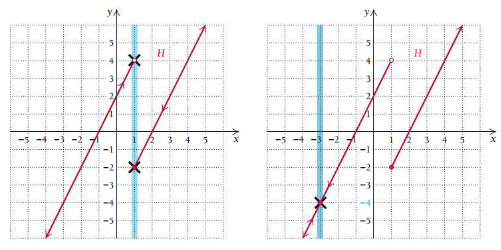
\includegraphics[width=0.6\textwidth]{ /home/mattw/niu/Math211/figures/ksnip_20230921-191506.png }
\caption*{wall method}
\end{figure}
\bigbreak \noindent
However, for any other value a, $\displaystyle\lim_{x\to a }H(x)$ does exist. For example, as x approaches -3, we see in the graph to the right that the wall method gives -4 whether -3 is approached from the left or from the right. Thus,
$$\displaystyle\lim_{x\to -3 }H(x) = -4$$
\bigbreak \noindent
\ex{}{
  Consider the piecewise function defined as follows:
 $$
G(x)= \begin{cases}5, & \text { for } x=1 \\ x+1, & \text { for } x \neq 1\end{cases}
$$ 
\bigbreak \noindent
Graph the function, and find each of the following:
\bigbreak \noindent
$$\text{a) } G(1)\hspace{10mm} \text{b) } \displaystyle\lim_{x\to 1}G(x)$$
}
\sol{}
\bigbreak \noindent
The graph of G follows.
\begin{figure}[ht]
    \centering
    \incfig[1]{fg}
    %\caption{fg}
    %\label{fig:fg}
\end{figure}
\bigbreak \noindent
From the definition of G, we see that
$$G(1) = 5$$
\pagebreak

\noindent b) As inputs x approach 1 from the left, outputs $G(x)$ approach 2, so the limit from the left is 2. As inputs x approach 1 from the right, outputs G(x) also approach 2, so the limit from the right is 2. Both limits are the same, so
$$\displaystyle\lim_{x\to 1}G(x) = 2$$
\bigbreak \noindent
\nt{
  Note that the limit, 2, is not the same as the function value of 1.
}
\begin{figure}[ht]
\centering
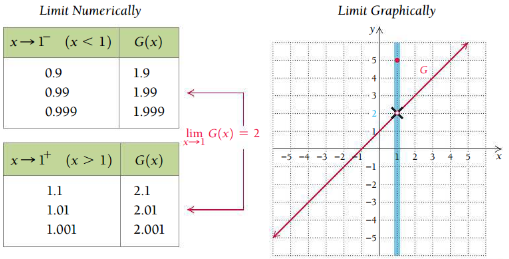
\includegraphics[width=0.65\textwidth]{ /home/mattw/niu/Math211/figures/IV.png }
\end{figure}
\bigbreak \noindent \bigbreak \noindent
\subsection{Limits Involving Infinity}
\bigbreak \noindent
Limits also help us understand the role of infinity with respect to some functions.
\bigbreak \noindent
\ex{}{
  Let $f(x) = \frac{1}{x-2}$
  \bigbreak \noindent
  \begin{enumerate}
    \item Find $\displaystyle\lim_{x\to 2^-}f(x)$
    \item Find $\displaystyle\lim_{x\to 2^+}f(x)$
    \item Does $\displaystyle\lim_{x\to 2}f(x)$ exist? Why or why not?
  \end{enumerate}
  \bigbreak \noindent
  \vspace{2mm}

  \sol{}
  \bigbreak \noindent
  a) as x approaches 2 from the left, f(x) decreases without bound. We conclude that the left-hand limit is $-\infty$; that is:
  $$\displaystyle\lim_{x\to 2}f(x) = -\infty$$
  \bigbreak \noindent
  b) as x approaches 2 from the right, f(x) increases without bound. We conclude that the right-hand limit is $\infty$ that is:
  $$\displaystyle\lim_{x\to 2}f(x) = \infty$$
  \bigbreak \noindent
  c) Since the left-hand and right-hand limits are not the same, we conclude that $\displaystyle\lim_{x\to 2}f(x)$ does not exist.
}
\pagebreak

\ex{}{
  Consider the function $f$ given by
$$f(x) = \frac{3x-5}{x-2}$$
\bigbreak \noindent
\centerline{ a) $\displaystyle\lim_{x\to 3}f(x) \hspace{5mm} \text{b) }\displaystyle\lim_{x\to 2}f(x) \hspace{5mm} \text{c) }\displaystyle\lim_{x\to -\infty}f(x) \hspace{5mm} \text{d) }\displaystyle\lim_{x\to \infty}f(x)$}
\bigbreak \noindent
a) We can use direct substitution for this one,

$$ \frac{3(3)-5}{3-2} = \frac{4}{1} = 4$$
The limit as x approaches 3 is 4
\bigbreak \noindent
b) As $x\to 2$ from the right, f(x) goes to $\infty$, as  $ x\to 2$ from the left, f(x) goes to $-\infty$, so this limit DNE
\bigbreak \noindent
c) If we were to graph this rational function, it would show that as $x\to -\infty$, x approaches 3. therefore,
$$\displaystyle\lim_{x\to -\infty}f(x) = 3$$
\bigbreak \noindent
d) As x approaches negative infinity, much as in part (c), the outputs again approach 3. Thus,
$$\displaystyle\lim_{x\to \infty}f(x) = 3$$
\centerline{\incfig[1]{ratfunct}}
}
\bigbreak \noindent
\begin{large}
  \textbf{Section Summary} 
\end{large}
\bigbreak
\begin{minipage}{0.4\textwidth}
\begin{itemize}
  \item The notation $x \rightarrow a^{-}$represents a sequence of numbers that approach a limit value $a$ from the left. The notation $x \rightarrow a^{+}$represents a sequence of numbers that approach a limit value $a$ from the right.
  
  \item The limit of $f(x)$, as $x$ approaches $a$, is written $\lim _{x \rightarrow a} f(x)=L$. This means that as the values of $x$
approach $a$, the corresponding values of $f(x)$ approach $L$. The value $L$ must be a unique real number.
\end{itemize}	
\end{minipage}
\begin{minipage}{0.5\textwidth}
\begin{itemize}
  \item A left-hand limit is written $\lim _{x \rightarrow a^{-}} f(x)$. Values of $x$ approach $a$ from the left, that is, $x<a$.
  \item A right-hand limit is written $\lim _{x \rightarrow a^{+}} f(x)$. Values of $x$ approach $a$ from the right, that is, $x>a$.
\end{itemize}	
\end{minipage}
\pagebreak
\section*{1.2 - Algebraic Limits and Continuity}
\bigbreak \noindent \bigbreak \noindent
\subsection*{Algebraic Limits}
\bigbreak \noindent
Consider the functions given by $f(x) = x, g(x) = 3, and F(x) = x+3$, displayed in the following graphs.
\vspace{3mm}

\nt{
  Notice that function F is the sum of the functions $f$ and $g$.
}
\begin{figure}[ht]
\centering
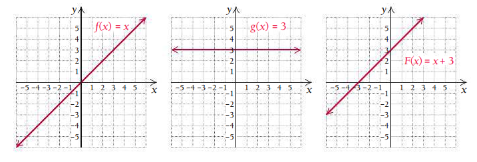
\includegraphics[width=0.9\textwidth]{ /home/mattw/niu/Math211/figures/img.png }
\end{figure}
\bigbreak \noindent
Suppose we are interested in the limit of f(x), g(x), and F(x) as x approaches 2. In Section 1.1, we learned numerical and graphical techniques that can be used top show that

$$\displaystyle\lim_{x\to 2}f(x)=2 \hspace{5mm} \displaystyle\lim_{x\to 2}g(x)=3 \hspace{5mm} \displaystyle\lim_{x\to 2}F(x)=5$$
\vspace{3mm}

\noindent These techniques work for any value of a in $\displaystyle\lim_{x\to a}f(x)$. For example, if we choose $a=-1$, we can compute the following limits:
$$\displaystyle\lim_{x\to -1}f(x)=-1 \hspace{5mm} \displaystyle\lim_{x\to -1}g(x)=3 \hspace{5mm} \displaystyle\lim_{x\to -1}F(x)=2$$
\bigbreak \noindent
From these results, the following observation can be made:
\begin{enumerate}
  \item For any real number a, $\displaystyle\lim_{x\to a }x=a$ 
  \item For any real number a, $\displaystyle\lim_{x\to a }3= 3$
\end{enumerate}
\bigbreak \noindent
Recalling that F(x) = f(x) + g(x), we make this reasonable conclusion:
\vspace{3mm}

\hspace{-6mm}3. For any real number a, $\displaystyle\lim_{x\to a }(x+3) = a + 3$
\bigbreak \noindent
\pagebreak
\subsection*{Limit Properties}
\bigbreak \noindent
if $\displaystyle\lim_{x\to a}f(x) = L$ and $\displaystyle\lim_{x\to a }g(x) = M$, and c is any constant, then we have the following limit properties.
\bigbreak \noindent
\begin{mdframed}
L1. The limit of a constant function is the constant itself:
$$
\lim _{x \rightarrow a} c=c .
$$
L2. The limit of a power function is the limit of the base, raised to that power.
$$
\lim _{x \rightarrow a}[f(x)]^n=\left[\lim _{x \rightarrow a} f(x)\right]^n=L^n, \quad \text { and } \quad \lim _{x \rightarrow a} \sqrt[n]{f(x)}=\sqrt[n]{\lim _{x \rightarrow a} f(x)}=\sqrt[n]{L}
$$
In tL3. The limit of a sum or difference is the sum or difference of the limits:
$$
\lim _{x \rightarrow a}[f(x) \pm g(x)]=\lim _{x \rightarrow a} f(x) \pm \lim _{x \rightarrow a} g(x)=L \pm M .
$$
L4. The limit of a product is the product of the limits:
$$
\lim _{x \rightarrow a}[f(x) \cdot g(x)]=\left[\lim _{x \rightarrow a} f(x)\right] \cdot\left[\lim _{x \rightarrow a} g(x)\right]=L \cdot M .
$$
L5. The limit of a quotient is the quotient of the limits:
$$
\lim _{x \rightarrow a} \frac{f(x)}{g(x)}=\frac{\lim _{x \rightarrow a} f(x)}{\lim _{x \rightarrow a} g(x)}=\frac{L}{M}, \quad \text { assuming } M \neq 0 .
$$
L6. The limit of a constant times a function is the constant times the limit of the function:
$$
\lim _{x \rightarrow a} c \cdot f(x)=c \cdot \lim _{x \rightarrow a} f(x)=c \cdot L .
$$
Property L6 combines L1 and L4 but is stated separately because it is used so frequently.he case of the power, we must have $L \neq 0$ if $n$ is negative, and in the case of the root, we must have $L \geq 0$ if $n$ is an even integer.
\end{mdframed}
\bigbreak \bigbreak \noindent
Using the limit properties, we can solve the following problem:

$$\displaystyle\lim_{x\to 4}(x^2-3x+7)$$
\bigbreak \noindent
By limit Property L2,
$$\displaystyle\lim_{x\to 4} = \left[ \displaystyle\lim_{x\to 4}x\right]^2 = 4^2 = 16$$ 
By limit Property L6,
$$\displaystyle\lim_{x\to 4}(-3x) = -3 \cdot \displaystyle\lim_{x\to 4}x = -3 \cdot 4 = -12$$
By limit Property L1,
$$\displaystyle\lim_{x\to 4}7 = 7$$
By limit Property L3 to combine these results, we have
$$\displaystyle\lim_{x\to 4 }(x^2-3x+7) = 16-12+7 = 11$$
\pagebreak
\thm{Limits of Rational Functions}{
  For any rational function F, with a in the domain of F,
  $$\displaystyle\lim_{x\to a }F(x) = F(a)$$
}
\bigbreak \noindent
\nt{
Rational functions include all polynomial functions (which include constant functions and linear functions) and ratios composed of such functions. Thus, the Limit Properties allow us to evaluate limits of rational functions, for values in a functions domain, quickly without tables or graphs, as illustrated in the following examples.
}
\bigbreak \noindent
\ex{}{

  Find $\displaystyle\lim_{x\to 2 }(x^4-5x^3+x^2-7)$
  \bigbreak \noindent
  \sol
  \bigbreak \noindent
  $$\displaystyle\lim_{x\to 2 }(x^4-5x^3+x^2-7) = 2^4-5(2)^3+2^2-7$$
  $$ = -27$$
}
\bigbreak \noindent \bigbreak \noindent
\ex{}{
  Let r(x) = $ \frac{x^2-x-12}{x+3}$
  \vspace{3mm}

  Find $\displaystyle\lim_{x\to -3}r(x)$
  \bigbreak \noindent
  \sol{}
  Since -3 is not in the domain of r(x), we cannot use direct substitition to find the limit of $x \to -3$
  \bigbreak \noindent
  We can however simplify by factoring the numerator,
  $$\frac{x^2-x-12}{x+3} = \frac{(x+3)(x-4)}{x+3}$$
  we can simplify futher, since x+3 can be cancelled out of the equation. After cancelling we are left with
  $$ x-4$$
  Therefore,
  $$\displaystyle\lim_{x\to -3}(x-4) = (-3) + 4 = -7$$
  $$\displaystyle\lim_{x\to -3}r(x)=-7$$
  
}
\pagebreak
\begin{mdframed}
  
\noindent The graph of $r$ is a line with a "hole" at $(-3,-7)$. Even though $r(-3)$ does not exist, the limit does exist since we are concerned about the behavior of $r(x)$ as $x$ approaches -3 . 
\vspace{3mm}

\noindent The decision to simplify was made by noting that $\left[(-3)^2-(-3)-12\right] /[(-3)+3]=0 / 0$. This indeterminate form indicates that the polynomials in the numerator and the denominator share a common factor, in this case, $(x+3)$. The $0 / 0$ form is a hint that a limit may exist. 
\vspace{3mm}

\noindent Look for ways to simplify algebraically, or use a table or a graph to determine a limit in cases like this.
\vspace{5mm}

\noindent A common error in determining limits is to assume that all limits can be found by direct evaluation. Students may attempt to find the limit of a function like the one in example 1.9, get a zero in the denominator, and then mistakenly conclude that the limit does not exist. 
\vspace{3mm}

\noindent Remember, finding a limit as $x$ approaches $a$ focuses on $x$ close to $a$, not at $a$. As Example 5 shows, a function may not be defined at a certain $a$-value, but its limit as $x \rightarrow a$ may still exist.
\bigbreak \noindent
The Limit Properties can also be used to evaluate limits of rational functions as $x$ approaches infinity.
\end{mdframed}
\bigbreak \noindent
\noindent
Find $\displaystyle\lim_{x\to \infty}\frac{x^2+4x-5}{2x^2+x+1}$
\bigbreak \noindent
\nt{
  for rational functions, if the function is bottom heavy, then the limit will always be 0.
  \bigbreak \noindent
  for example, in f(x) = $\frac{1}{x}$ notice that as x gets larger, the value for f(x) gets smaller, hence, bottom heavy.
  \bigbreak \noindent
  For finding the limit as $x \to \infty$ for a rational function, what we can do is simply multiply the top and bottom by the highest degree found in the function. for example if the highest degree is $x^2$, we multiply top and bottom by $\frac{1}{x^2}$
}
\bigbreak \noindent
So for this problem, we can multiply the top and bottom by $\frac{1}{x^2}$
$$\displaystyle\lim_{x\to \infty}\frac{x^2+4x-5}{2x^2+x+1} = \displaystyle\lim_{x\to \infty}\frac{x^2+4x-5}{2x^2+x+1}\cdot \frac{\frac{1}{x^2}}{\frac{1}{x^2}}$$

$$ = \frac{1 + \frac{4}{x} -\frac{5}{x^2}}{2 + \frac{1}{x} + \frac{1}{x^2}}$$
Now if we were to break this up into many limits using the properties of limits, we would end up with,
$$ \frac{1+0+0}{2+0+0} = \frac{1}{2}$$
\text{ this is because all the terms that are bottom heavy have a limit of 0 when x goes to $\infty$}
Therefore,
$$\displaystyle\lim_{x\to\infty}f(x) = \frac{1}{2}$$
\bigbreak \noindent
  The limit properties can be used to show that if $f(x) = \frac{ax^m + \ldots}{bx^n \ldots}$, then
  \begin{itemize}
    \item $\displaystyle\lim_{x\to \pm\infty}f(x) = \frac{a}{b}$ if m = n
    \item $\displaystyle\lim_{x\to\pm\infty}f(x) = 0$ if $m < n$
    \item and, $\displaystyle\lim_{x\to\pm\infty}f(x)$ does not exist if $m > n$
  \end{itemize}
\pagebreak
In calculus, we often consider expressions containing more than one variable.
Consider the following example,
$$\displaystyle\lim_{h\to 0}(3x^2+3xh+h^2)$$
\bigbreak \noindent
We treat x as a constant since we are interested only in how the expression changes as h approaches 0. We use the Limit Properties to find that
$$\displaystyle\lim_{h\to 0}(3x^2+3xh+h^2) = 3x^2 + 3x(0) + (0)^2 $$
$$ = 3x^2$$
\subsection*{Continuity}
The following graphs of continuous functions. For now, we use an intuitive definition of continuity, which we will soon refine.
\begin{figure}[ht]
\centering
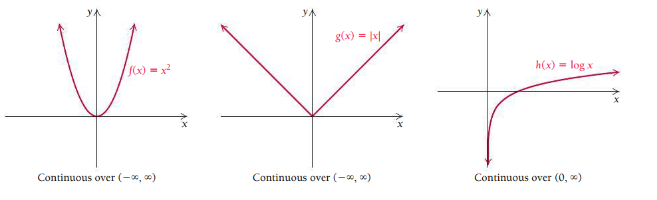
\includegraphics[width=0.9\textwidth]{ /home/mattw/niu/Math211/figures/ksnip_20230926-205010.png}
\end{figure}
\bigbreak \noindent
\nt{
  Note that there are no ``jumps'' or ``holes'' in the graphs. We say that a function is continuous over, or on, some interval, of the real number line if its graph can be traced without lifting a pencil off the graph. If there is any point in an interval where a ``jump'' or a ``hole'' occurs, then we say that the function is \textbf{not continuous, or is \textbf{discontinuous}, over that interval. The function F, G, and H in the following graphs are examples of functions that are not continuous over $(-\infty,\infty)$}
}
\begin{figure}[ht]
\centering
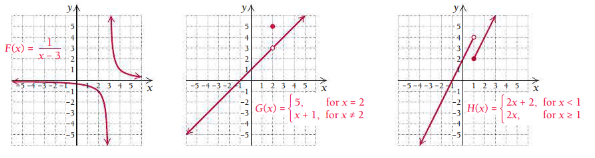
\includegraphics[width=0.9\textwidth]{ /home/mattw/niu/Math211/figures/ksnip.png }
\end{figure}
\bigbreak \noindent
In each case, the graph cannot be traced without lifting the pencil off the graph.
\vspace{1.5mm}

\noindent However, each case represents a different situation.

\pagebreak

\hspace{-14mm}\begin{minipage}{0.45\textwidth}
\begin{itemize}
  \item F is not continuous over $(-\infty, \infty)$ because 3 is not in the domain of F. Thus, there is no point to trace at x = 3. Note that F is continuous for all x in its domain, $(-\infty, 3) \cup (3,\infty)$
  \item G is not continuous over $(-\infty,\infty)$ because it is not continuous a $ x=1$. To see this, trace the graph and note that as x apporaches 1 from the left, H(x) approaches 4. However, as $x \to 1$ from the right, H(x) approaches 2. Note that 
  \item Each of the above graphs has a point of discontinuity. The graph of $F$ is discontinuous at 3 , because $x=3$ is not in the domain of $F ; G$ is discontinuous at 2 , because $\lim _{x \rightarrow 2} G(x) \neq G(2)$; and $H$ is discontinuous at 1 , because $\lim _{x \rightarrow 1} H(x)$ does not exist.
\end{itemize}
\end{minipage}
\hspace{8mm}\begin{minipage}{0.6\textwidth}
\thmcon{
  \textbf{\underline{Defintion}}
  \vspace{3mm}

  A function $f$ is continuous at x = a if:
  \begin{enumerate}
    \item f(a) exists \hspace{10mm} (The input a is in in the domain of $f$)
    \item $\displaystyle\lim_{x\to a }f(x)$ exists \hspace{5mm} (The limit as x approaches a exists)
    \item $\displaystyle\lim_{x\to a }f(x) = f(a)$ \hspace{3.5mm} (The limit is the same as the output)
  \end{enumerate}
  \bigbreak \noindent
  A function is continuous over an open interval if it is coninuous at each point a in i. IF f is not continuous at x = a, we say that f is discontinuous, or has a discontinuity, at x = a

}	
\end{minipage}
\bigbreak \noindent \bigbreak \noindent
\hrule
\bigbreak
\ex{}{
  Determine whether the function given by
  $$ f(x) = 2x + 3$$
  is continuous at x = 4
  \bigbreak \noindent
  \sol{}
\bigbreak \noindent
 1. f(4) exists (the input 4 is in the domain of $f$ )
 \bigbreak \noindent 
 2. $\displaystyle\lim_{x\to 4}f(x)$ exists, 
 $$\displaystyle\lim_{x\to 4}f(x) = 11$$
 3. $\displaystyle\lim_{x\to 4}f(x) = 11 = f(4)$
 \bigbreak \noindent
 Since $\displaystyle\lim_{x\to 4}f(x) = f(4)$ the function is indeed continuous at x = 4.
 
  }
\bigbreak \noindent \bigbreak \noindent
\ex{}{
  Is the function F, given by
  $$
F(x)= \begin{cases}\frac{x^2-16}{x-4}, & \text { for } x \neq 4 \\ 7, & \text { for } x=4\end{cases}
$$ 
continuous at x = 4? Why or why not?
\bigbreak \noindent
\sol{}
\bigbreak \noindent
For F to be continuous at 4, we must have $\displaystyle\lim_{x\to 4}F(x) = F(4).$ We are given F(4) = 7. To find $\displaystyle\lim_{x\to 4}F(x)$, note that, for $x \neq 4$,
$$\frac{x^2-16}{x-4} = \frac{(x+4)(x-4)}{x-4} = x+ 4$$
Thus,
$$\displaystyle\lim_{x\to 4 }F(x) = 4 + 4 = 8$$
We see that F is not continuous at x = 4 since
$$\displaystyle\lim_{x\to 4}F(x) \neq F(4)$$


}
\bigbreak \noindent
\section*{1.3 - Average Rates of Change}
\begin{mdframed}
  \vspace{2mm}

  A \textit{rate,} or \textit{rate of change}, is a ratio of two quantities. For example, if you drive 110 mi over a 2-hr period, then your \textit{average rate of change} in distance (miles) per unit of time (hours) over the 2-hr period is $\frac{110}{2 hr}$, or 55 mi/hr. Suppose that at one instant during your drive, you glance at the speedometer and see that at that moment you are traveling at 65 mi/hr. This is an \textit{instantaneous rate of change} These are two different, yet related, concepts. To understand instantaneous rate of change. we first need to develop a solid understanding of average rate of change.
  \vspace{2mm} 

\end{mdframed}
\bigbreak \noindent \bigbreak \noindent
\ex{}{
  State the average rate of change for each situation. Be sure to include units.
  \begin{enumerate}
    \item Jan rode a bicycle 30 miles in 3 hours. 
      \subitem $\frac{30 mi}{3 hr} = 10\frac{mi}{hr}$
    \item It snowed 12 in. between midnight and 8 a.m.
      \subitem $\frac{12 in.}{8hr} = 1.5\frac{in}{hr}$
    \item Sue earned \$250 from selling 8 pieces of jewelry.
      \subitem $\frac{250 dollars}{8 pieces} = 31.25 \frac{\text{dollars}}{\text{piece}}$
  \end{enumerate}
}
\bigbreak \noindent
\ex{}{
  The graph below shows fourth-quarter revenue from Groupon from 2012 to 2017, rounded to the nearest million dollars.
  \begin{enumerate}
    \item How much did revenue increase between the fourth quarter of 2014 and the fourth quarter of 2015? 
      \item What was the average change in fourth-quarter revenue between 2013 and 2016?
  \end{enumerate}
}
\pagebreak
\section*{1.5 - Leibniz Notation and the Power and Sum-Difference Rules}
To find derivatives of functions instead of using the formula

$$ f'(x) = \displaystyle\lim_{h\to 0}\frac{f(x+h) - f(x)}{h}$$
We can use

$$\frac{dy}{dx}$$
\bigbreak \noindent
This notation is called \textit{leibniz notation}, using this notation we often write the derivative as

$$\frac{dy}{dx} = f'(x)$$
\bigbreak \noindent
It is important to note that the d's are not variables and that

$$\frac{dy}{dx} \neq \frac{y}{x}$$
\bigbreak \noindent
We can also express the derivative of $f$ as
$$\frac{dy}{dx}f(x)$$
\bigbreak \noindent
For example

$$ \frac{d}{dx}(x^2) = 2x, \hspace{5mm} \frac{d}{dx}(x^3) = 3x^2, \hspace{5mm}  \frac{d}{dx}(\frac{1}{x}) = -\frac{1}{x^2}$$
\bigbreak \noindent
\subsection*{The Power Rule}
\bigbreak \noindent
\begin{mdframed}
For any real number k, if y = $x^k$, then
$$ \frac{d}{dx}x^k = k \cdot x^{k-1}$$
\vspace{2mm}
\end{mdframed}
\bigbreak \noindent\bigbreak \noindent
$$ \frac{d}{dx}x^2 = 2x$$ 

$$ \frac{d}{dx}x^3 = 3x^2$$

$$ \frac{d}{dx}x^4 = 4x^3$$

$$ \frac{d}{dx}x^{-1} = -1x^{-2}$$

$$ \frac{d}{dx}x^{\frac{1}{2}} = \frac{1}{2}x^{-\frac{1}{2}}$$
\pagebreak
\begin{mdframed}
 Differentiate each of the following with respect to x 
 $$ y = x^5 \hspace{10mm} y = x \hspace{10mm}y = x^{-4}$$
\end{mdframed}
\bigbreak \noindent
1) $ \frac{d}{dx}x^5 
$$= 5x^4$
\bigbreak \noindent
2) $ \frac{d}{dx}x = 1$
\bigbreak \noindent
3) $ \frac{d}{dx}x^{-4} \hspace{5mm} \rightarrow \hspace{5mm} -4 \cdot x^{-4-1} \hspace{5mm} \rightarrow \hspace{5mm} -4x^{-5}, \hspace{5mm} \rightarrow \hspace{5mm} -4 \cdot\frac{1}{x^5} = -\frac{4}{x^5}$
\bigbreak \noindent \bigbreak \noindent
The Power Rule also allows us to differentiate expression with rational exponents
\bigbreak \noindent
For example, 
\bigbreak \noindent
a) $\frac{d}{dx}\sqrt[5]{x}$
$$ \frac{1}{5} \cdot x^{-\frac{4}{5}}$$

$$\frac{1}{5} \cdot \frac{1}{x^{\frac{4}{5}}}$$

$$= \frac{1}{5\sqrt[5]{x^4}}$$
\bigbreak \noindent
b) $\frac{d}{dx}x^{0.7}$
  $$ \frac{d}{dx}0.7x^{-0.3}$$

  $$\frac{7}{10}\cdot\frac{1}{x^{0.3}}$$

  $$ = \frac{7}{10x^{0.3}}$$
  \bigbreak \noindent
  \subsection*{The Derivative of a Constant Function}
  Consider the constant function given by $f(x) = c$. Note that the slope of the tangent line at each point on its graph is 0.
\begin{figure}[ht]
\centering
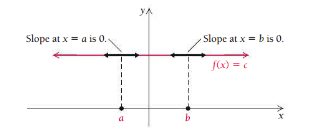
\includegraphics[width=0.8\textwidth]{ /home/mattw/niu/Math211/latexdocs/figures/dx.png }
\end{figure}

\pagebreak
\noindent This suggests the following theorem
\bigbreak \noindent
\thm{}{
  The derivative of a constant function is 0. That is, $ \frac{d}{dx}c = 0$
}
\bigbreak \noindent
Differentiate with respect to x:
$$y=7; \hspace{20mm} y = \pi^2$$
\sol
\bigbreak \noindent
\begin{minipage}{0.5\textwidth}
$$ \frac{d}{dx}(7) = 0$$
\end{minipage}
\begin{minipage}{0.45\textwidth}
$$ \frac{d}{dx}\pi^2 = 0$$	
\end{minipage}
\bigbreak \noindent
\subsection*{The Derivative of a Constant Times a Function}
\thm{}{
  The derivative of a constant times a function is the constant times the derivative of the function. Using derivative notation, we can write this as
  $$ \frac{d}{dx}\bigg[c\cdot f(x)\bigg] = c \cdot \frac{d}{dx}f(x)$$
}
\bigbreak \noindent
Find each of the following derivatives:
$$ \frac{d}{dx}7x^4; \hspace{10mm} \frac{d}{dx}(-5\sqrt{x}); \hspace{10mm} \frac{d}{dx}\left(\frac{1}{5x^2}\right)$$
\bigbreak \noindent \bigbreak \noindent
\textbf{1.} 
$$ \frac{d}{dx}7x^4$$
$$ 7 \cdot 4x^3$$
$$ 28x^3$$
\bigbreak \noindent
\textbf{2.}
$$ \frac{d}{dx}(-5\sqrt{x})$$
$$ -5x^{\frac{1}{2}}$$
$$ -5 \cdot \frac{1}{2}x^{-\frac{1}{2}}$$
$$-\frac{5}{2}x^{-\frac{1}{2}}$$
\bigbreak \noindent
\textbf{3.}
$$ \frac{d}{dx}\left(\frac{1}{5x^2}\right)$$         
$$ \frac{1}{5}x^{-2}$$
$$ \frac{1}{5}\cdot \frac{d}{dx}x^{-2}$$
$$ \frac{1}{5} \cdot -2x^{-3}$$
$$ -\frac{2}{5}x^{-3} = \frac{-2}{5x^3}$$
\pagebreak
\section*{The Derivative of a Sum or a Difference}
\bigbreak \noindent
\textbf{Sum.} \hspace{15mm} The derivative of a sum is the sum of the dervatives:
$$ \frac{d}{dx}\left[f(x) + g(x)\right] = \frac{d}{dx}f(x) + \frac{d}{dx}g(x)$$
\bigbreak \noindent
\textbf{Difference.} \hspace{6mm} The derivative of a difference is the difference of the derivatives:
$$ \frac{d}{dx}\left[f(x) - g(x) \right] = \frac{d}{dx}f(x) - \frac{d}{dx}g(x)$$
\bigbreak \noindent \bigbreak \noindent
Find each of the following derivatives
\bigbreak \noindent
$$ \textbf{1.} \ \  \frac{d}{dx}(5x^3 -7) \hspace{20mm} \textbf{2.} \ \ \frac{d}{dx}(24x -\sqrt{x} + \frac{5}{x})$$
\bigbreak \noindent
\textbf{1.}
$$ \frac{d}{dx}5x^3 - \frac{d}{dx}7$$
$$ 5 \cdot 3x^2 - 0$$
$$ 15x^2$$
\bigbreak \noindent
\textbf{2.}
$$ \frac{d}{dx}24x - \frac{d}{dx}\sqrt{x} + \frac{d}{dx}\left(\frac{5}{x}\right)$$
$$ 24 - \frac{1}{2}x^{-\frac{1}{2}} + 5 \cdot -1x^{-2}$$
$$ 24 - \frac{1}{2\sqrt{x}} + 5 \cdot -\frac{1}{x^2}$$
$$ 24 - \frac{1}{2\sqrt{x}} - \frac{5}{x^2}$$
\bigbreak \bigbreak \noindent
\section*{Slopes of Tangent Lines}
It is important to be able to determine points at which the tangent line to a curve has a certain slope, that is, points at which the derivative, or rate of change, has a certain value.
\bigbreak \noindent \bigbreak \noindent
\q{}
 Find any points on the graph of $f(x) = -x^3 + 6x^2$ at which the tangent line is horizontal; the tangent line has slope 9
 \bigbreak \noindent \bigbreak \noindent
 Find $\frac{d}{dx}f(x)$
 $$ \frac{d}{dx}\left[-x^3 + 6x^2\right]$$
 $$ -3x^2 + 12x$$
 \bigbreak \noindent
 Set $ \frac{d}{dx}f(x) = 0$
 $$ -3x^2 +12x = 0$$

 \pagebreak
 \noindent Solve for x
 $$ -3x(x-4) = 0$$
 $$ -3x = 0 \hspace{8mm}or \ \  \  \ \ x -4 = 0$$
 $$ x = 0 \hspace{7mm} or \ \ \ \ \ x = 4$$
 \bigbreak \noindent
 Find the y-values
$$ f(0) = -(0)^3 + 6(0)^2 = 0$$
$$ f(4) = -(4)^3 + 6(4)^2 = 32$$
\bigbreak \noindent \bigbreak \noindent
Thus, the points where the tangent line is horizontal are

$$ \vspace{-3mm}\hspace{-5mm}(0,0) \hspace{5mm} (4,32)$$
\begin{figure}[ht]
    \centering
    \incfig[1]{tangent}
    %\caption{tangent}
    %\label{fig:tangent}
\end{figure}
\bigbreak \noindent

To find where the tangent line has slope 9, set f'(x) = 9
$$ -3x^2 +12x = 9$$
$$ -3x^2 + 12x - 9 = 0$$
$$ -3(x^2 - 4x + 3) = 0$$
$$ -3(x-3)(x-1) = 0$$
$$ x - 3 = 0 \hspace{5mm} x -1 =0$$
$$ x=3,1$$
Solve for y,
$$ f(3) = -(3)^3 + 6(3)^2 = 27$$
$$ f(1) = -(1)^3 + 6(1)^2 = 5$$
\bigbreak \noindent
So, the tangent line at (3,27) and (1,5) have a slope of 9.
\pagebreak
\section{1.6 - The Product and Quotient Rules}
\subsection*{The product Rule}
Some functions are easily viewed as the product of two other functions. For example, $F(x) = (x^2 + 3x)\sqrt{x}$ is the product of $f(x) = x^2 +3x$ and $g(x) = \sqrt{x}$ However, as a rule, the derivative of a product is not the product of the derivatives.
\bigbreak \noindent \bigbreak \noindent
Let $F(x) = f(x) \cdot g(x)$. Then
$$ F'(x) = \frac{d}{dx}\left[f(x) \cdot g(x)\right]$$

$$ = f(x) \cdot \left[\frac{d}{dx}g(x) \right] + g(x) \cdot \left[\frac{d}{dx}f(x)\right]$$
\bigbreak \noindent
\q
Find  $ \frac{d}{dx}\left[(x^4 - 2x^3 - 7\right)\left(3x^2-5x\right)]$
\bigbreak \noindent \bigbreak \noindent
Using the formula 
$$\frac{d}{dx}[f(x) \cdot g(x)] = f(x) \frac{d}{dx}[g(x)] + g(x) \frac{d}{dx}[f(x)]$$
\bigbreak \noindent
We get,
$$(x^4 -2x^3 - 7)(6x-5) + (3x^2 - 5x)(4x^3 - 6x^2)$$
\bigbreak \noindent \bigbreak \noindent
\q
\bigbreak \noindent
Find $ \frac{d}{dx}\left[(x^2+4x-11)(7x^3 - \sqrt{x})\right]$
Using the formula
$$ \frac{d}{dx}[f(x) \cdot g(x)] = f(x) \frac{d}{dx}[g(x)] + g(x) \frac{d}{dx}[f(x)]$$
\bigbreak \noindent
We get,
$$\left(x^2 + 4x -11\right)\left(21x^2 - \frac{1}{2}x^{-\frac{1}{2}}\right) + \left(7x^3 - x^{\frac{1}{2}}\right)\left(2x+4\right)$$
\bigbreak \noindent \bigbreak \noindent
\section*{The Quotient Rule}
The derivative of a quotient is not the quotient of the derivatives. To see why, consider $x^5$ and $x^2$ and assume $x\neq 0$. The quotient $\frac{x^5}{x^2}$ is $x^3$, and the derivative of this quotient is $3x^2$
\bigbreak \noindent
Let $F(x) = \dfrac{f(x)}{g(x)}$.
\bigbreak \noindent
Then,
$$ F'(x) = \frac{d}{dx}\bigg[ \frac{f(x)}{g(x)}\bigg] = \frac{g(x) \frac{d}{dx}[f(x)] - f(x) \frac{d}{dx}[g(x)]}{[g(x)]^2}$$
\pagebreak
\q
\bigbreak \noindent
Differentiate f(x) = $\dfrac{1 + x^2}{x^3 + 1}$

\bigbreak \noindent \bigbreak \noindent
Using the formula
$$ \frac{d}{dx}\bigg[ \frac{f(x)}{g(x)}\bigg] = \frac{g(x) \frac{d}{dx}[f(x)] - f(x) \frac{d}{dx}[g(x)]}{[g(x)}^2$$

\bigbreak \noindent \bigbreak \noindent
We get
$$ \dfrac{dy}{dx} = \dfrac{\left(x^3+1\right)\left(2x\right) - \left(1+x^2\right)\left(3x^2\right)}{\left(x^3 + 1\right)^2}$$ 
\vspace{1mm}

  $$= \dfrac{-x^4 - 3x^2 + 2x}{\left(x^3 + 1\right)^2}$$
  \bigbreak \noindent \bigbreak \noindent
  \section*{Application of the Quotient Rule}  
  The total cost, total revenue, and total profit functions, discussed in Section R.4, pertain to the accumulated cost, revenue, and profit when x items are produced. Because of economies of scale and other factors, it is common for the cost, revenue (price), and profit for, say, the 10th item to differ from those for the 1000th item. For this reason, businesses often focus on average cost, revenue, and profit
  \bigbreak \noindent \bigbreak \noindent
  \thmcon{
    \textbf{\underline{Defintion}}
    \vspace{3mm}
  
    If C(x) is the cost of producing x items, then the average cost of producing x items is
    $$ \frac{C(x)}{x}$$
    \bigbreak \noindent
    If R(x) is the revenue from the sale of x items, then the average revenue from selling x items is 
    $$\frac{R(x)}{x}$$
    \bigbreak \noindent
    If P(x) is the profit from the sale of x items, then the average profit from selling x items is
    $$ \frac{P(x)}{x}$$
  }
  \bigbreak \bigbreak
  \pagebreak
\ex{}{
 Paulsen's Greenhouse finds that the cost, in dollars, of growing x hundred geraniums is modeled by 
 $$ C(x) = 200 + 100\sqrt[4]{x}$$
 \bigbreak \noindent
If revenue from the sale of x hundred geraniums is modeled by
$$ R(x) = 120 +90\sqrt{x}$$
\bigbreak \noindent
Find each of the following
\bigbreak \noindent
a) The average cost, average revenue, and average profit when 300 geraniums are grown and sold
\bigbreak \noindent
b) The rate at which the average profit is changing when 300 geraniums are grown and sold
\bigbreak \noindent
\sol{}
\bigbreak \noindent
a) We let $\bar{C}, \bar{R}$, and $\bar{P}$ represent average cost, average revenue, and average profit, respectively, Thus, 
$$ \bar{C}(x) = \dfrac{C(x)}{x} = \dfrac{200 + 100\sqrt[4]{x}}{x}$$

$$ \bar{R}(x) = \dfrac{R(x)}{x} = \dfrac{120 + 90\sqrt{x}}{x}$$

$$\bar{P}(x) = \dfrac{R(x) - C(x)}{x} = \dfrac{-80 + 90\sqrt{x} - 100\sqrt[4]{x}}{x}$$
\bigbreak \bigbreak\noindent
\textbf{a)}
$$\bar{C}(3)=\frac{200+100 \sqrt[4]{3}}{3}=\$ \text{110.54 per hundred geraniums;}$$
$$\bar{R}(3)=\frac{120+90 \sqrt{3}}{3}=\$ \text{91.96 per hundred geraniums;}$$
$$\bar{P}(3)=\frac{-80+90 \sqrt{3}-100 \sqrt[4]{3}}{3} \approx-\$ \text{18.57 per hundred geraniums}$$
\bigbreak \bigbreak \bigbreak \noindent
\textbf{b)}
\bigbreak \noindent
$$
\begin{aligned}
\bar{P}^{\prime}(x) & =\frac{d}{d x}\left[\frac{-80+90 x^{1 / 2}-100 x^{1 / 4}}{x}\right] \\
& =\frac{x\left(\frac{1}{2} \cdot 90 x^{1 / 2-1}-\frac{1}{4} \cdot 100 x^{1 / 4-1}\right)-\left(-80+90 x^{1 / 2}-100 x^{1 / 4}\right) \cdot 1}{x^2} \\
& =\frac{45 x^{1 / 2}-25 x^{1 / 4}+80-90 x^{1 / 2}+100 x^{1 / 4}}{x^2}=\frac{75 x^{1 / 4}-45 x^{1 / 2}+80}{x^2} \\
\bar{P}^{\prime}(3) & =\frac{75 \sqrt[4]{3}-45 \sqrt{3}+80}{3^2}=11.20 .
\end{aligned}
$$
}
\pagebreak
\section*{The Chain Rule}
Suppose that g(x) is a differentiable function of x. Then, for any real number k,
$$ \frac{d}{dx}\left[g(x)\right]^{k-1} = k\left[g(x)\right]^{k-1}\cdot \frac{d}{dx}g(x)$$
\bigbreak \noindent
\q
\bigbreak \noindent
Differentiate $y=(x^2 + 3)^2
\bigbreak \noindent
$$ \frac{d}{dx}\left(x^2+3\right)^2$$
$$ 2\left(x^2+3)^1 \cdot 2x$$
$$  4x\left(x^2 +3)$$

$$ 4x^3 + 12x$$ 
\bigbreak \noindent
\q
\bigbreak \noindent
Differentiate h(x) = 6\left(x^3 -5x+1\right)^{10}
\bigbreak \noindent
$$ \frac{d}{dx}6\left(x^3-5x+1\right)^{10}$$
$$6 \cdot 10\left(x^3 - 5x +1\right)^{9}\left(3x^2 -5\right)$$

$$ 60(x^3-5x+1)^9(3x^2-5)$$
\bigbreak \noindent
\q
\bigbreak \noindent
Differentiate y = (1 + x^3)^{\frac{1}{2}}
\bigbreak \noindent

$$ \frac{d}{dx} = \dfrac{1}{2}(1+x^3)^{\frac{1}{2} - 1 } \cdot 3x^2$$

$$ = \dfrac{3x^2}{2}\left(1 + x^3\right)^{\frac{-1}{2}} = \dfrac{3x^2}{2\sqrt{1 + x^3}}$$
\bigbreak \noindent
\q
\bigbreak \noindent
Differentiate $y = \dfrac{5}{ \left(1-x^2\right)^3}$
\bigbreak \noindent
$$ 5 \left(-3 \left(1 -x^2\right)^4 \left(-2x\right) \right)$$

$$ = \dfrac{30x}{ \left(1-x^2\right)^4}$$
\pagebreak
\q
\bigbreak \noindent
Differentiate $f(x) = (3x-5)^4 \left(7 -x\right)^{10}$
\bigbreak \noindent
$$ f'(x) = (3x - 5)^4 \cdot 10(7 - x)^9(-1) + (7-x)^{10} \cdot 4(3x-5)^3(3)$$
$$ = -10 (3x-5)^4(7-x^{9}) + (7 - x)^{10}\left[12(3x-5)^3\right]$$
\bigbreak \noindent
Factor out $2(3x-5)^3(7-x)^9$

$$= 2(3x-5)^3 (7-x)^9[-5(3x-5) + 6(7-x)]$$
$$ = 2(3x - 5)^3 (7-x)^9 (-15x+25+42-6x)$$

$$ 2(3x-5)^3(7-x)^9(67 - 21x)$$
\bigbreak \noindent
\q
\bigbreak \noindent
Differentiate $f(x) = \sqrt[4]{\dfrac{x+3}{x-2}}$
\bigbreak \noindent




\end{document}

